\documentclass[10pt, landscape]{article}
\usepackage[scaled=0.92]{helvet}
\usepackage{calc}
\usepackage{multicol}
\usepackage{ifthen}
\usepackage[a4paper,margin=5mm,landscape]{geometry}
\usepackage{amsmath,amsthm,amsfonts,amssymb}
\usepackage{color,graphicx,overpic}
\usepackage{hyperref}
\usepackage{newtxtext} 
\usepackage{enumitem}
\usepackage{amssymb}
\usepackage[table]{xcolor}
\usepackage{vwcol}
\usepackage{tikz}
\usetikzlibrary{arrows.meta}
\usetikzlibrary{calc}
\usepackage{mathtools}
\usepackage{nicematrix}
\usepackage[T1]{fontenc} %%% <--- NOTE THIS
% for relations
\usepackage{cancel}
\usepackage{ mathrsfs }
\usepackage{listings}
\usepackage{background}
\usepackage{epigraph}
\setlist{nosep}

\usepackage{etoolbox}
\makeatletter
\preto{\@verbatim}{\topsep=0pt \partopsep=0pt }
\makeatother

\backgroundsetup{
scale=1,
color=black,
opacity=0.4,
angle=0,
contents={}
% contents={
\includegraphics[width=\paperwidth,height=\paperheight]{image.png}}
}

\pdfinfo{
  /Title (MA2214.pdf)
  /Creator (TeX)
  /Producer (pdfTeX 1.40.0)
  /Author (Seamus)
  /Subject (Example)
  /Keywords (pdflatex, latex,pdftex,tex)}

\lstset{language=Java,keywordstyle={\bfseries \color{black}}}

% Turn off header and footer
\pagestyle{empty}

\newenvironment{tightcenter}{%
  \setlength\topsep{0pt}
  \setlength\parskip{0pt}
  \begin{center}
}{%
  \end{center}
}

% redefine section commands to use less space
\makeatletter
\renewcommand{\section}{\@startsection{section}{1}{0mm}%
                                {-1ex plus -.5ex minus -.2ex}%
                                {0.5ex plus .2ex}%x
                                {\normalfont\large\bfseries}}
\renewcommand{\section}{\@startsection{section}{2}{0mm}%
                                {-1explus -.5ex minus -.2ex}%
                                {0.5ex plus .2ex}%
                                {\normalfont\normalsize\bfseries}}
\renewcommand{\subsection}{\@startsection{subsection}{3}{0mm}%
                                {-1ex plus -.5ex minus -.2ex}%
                                {1ex plus .2ex}%
                                {\normalfont\small\bfseries}}%
\renewcommand{\familydefault}{\sfdefault}
\renewcommand\rmdefault{\sfdefault}
% makes nested numbering (e.g. 1.1.1, 1.1.2, etc)
\renewcommand{\labelenumii}{\theenumii}
\renewcommand{\theenumii}{\theenumi.\arabic{enumii}.}
\renewcommand\labelitemii{•}
%  for logical not operator
\renewcommand{\lnot}{\mathord{\sim}}
\renewcommand{\bf}[1]{\textbf{#1}}
\newcommand{\abs}[1]{\vert #1 \vert}
\newcommand{\Mod}[1]{\ \mathrm{mod}\ #1}

\makeatother
\definecolor{myblue}{cmyk}{1,.72,0,.38}
\everymath\expandafter{\the\everymath \color{myblue}}
% Define BibTeX command
\def\BibTeX{{\rm B\kern-.05em{\sc i\kern-.025em b}\kern-.08em
    T\kern-.1667em\lower.7ex\hbox{E}\kern-.125emX}}
\let\iff\leftrightarrow
\let\Iff\Leftrightarrow
\let\then\rightarrow
\let\Then\Rightarrow

% Don't print section numbers
\setcounter{secnumdepth}{0}

\setlength{\parindent}{0pt}
\setlength{\parskip}{0pt plus 0.5ex}
%% this changes all items (enumerate and itemize)
\setlength{\leftmargini}{0.5cm}
\setlength{\leftmarginii}{0.5cm}
\setlist[itemize,1]{leftmargin=2mm,labelindent=1mm,labelsep=1mm}
\setlist[itemize,2]{leftmargin=4mm,labelindent=1mm,labelsep=1mm}

%My Environments
\newtheorem{example}[section]{Example}
% -----------------------------------------------------------------------

\begin{document}
\raggedright
\footnotesize
\begin{multicols*}{3}

% multicol parameters
% These lengths are set only within the two main columns
\setlength{\columnseprule}{0.25pt}
\setlength{\premulticols}{1pt}
\setlength{\postmulticols}{1pt}
\setlength{\multicolsep}{1pt}
\setlength{\columnsep}{2pt}

\begin{center}
    \fbox{%
        \parbox{0.8\linewidth}{\centering \textcolor{black}{
            {\Large\textbf{MA2214}}
            \\ \normalsize{AY25/26 Sem 1}}
            \\ {\footnotesize \textcolor{myblue}{by ngmh}} 
        }%
    }
\end{center}

\section{Basic Counting Principles}

\textbf{r-Permutation} An r-permutation of $A$ is a way of arranging any $r$ of the objects of $A$ in a row, with number denoted as $P_r^n=\frac{n!}{(n-r)!}$ by MP.

\textbf{Principle of Division} If we can partition instances of an event $E$ into disjoint r-element groups which each gives rise to a unique $E'$, then $|E'|=\frac{|E|}{r}$.

\textbf{Circular Permutation} An r-circular permutation of $A$ is a circular permutation of $r$ distinct objects taken from $A$, denoted $Q_r^n=\frac{P_r^n}{r}$.

\textbf{Combination} An r-combination of $A$ is an r-element subset of $A$, denoted by $C_r^n={n \choose r}=\frac{P_r^n}{r!}=\frac{n!}{r!(n-r)!}$. Additionally, ${n \choose r}={n \choose n-r}$.

\textbf{Combinatorial Identities}
\begin{itemize}
    \item ${n \choose r} = {n-1 \choose r-1}+{n-1 \choose r}$ (Either take the current element, or choose $r$ from the set without the current element)
    \item ${n \choose r} = \frac{n}{r}{n-1 \choose r-1}$ (Move $r$ over, then LHS becomes choosing $r$ then a leader while RHS becomes choosing the leader then remaining $r-1$)
    \item ${n \choose r} = \frac{n-r+1}{r}{n \choose r-1}$, ${n \choose r}=\frac{n}{n-r}{n-1 \choose r}$, ${n \choose m}{m \choose r}={n \choose r}{n-r \choose m-r}$
\end{itemize}

\textbf{Principle of Inclusion and Exclusion} $|A_1 \cup A_2 \cup... \cup A_q|=\sum_{i=1}^q |A_i|-\sum_{i<j}|A_i \cap A_j|+\sum_{i<j<k}|A_i\cap A_j \cap A_k|...+(-1)^{q-1}|A_1\cap...\cap A_q|$

\textbf{Euler's $\varphi$ Function} $\varphi(n)$ denotes the number of integers between $1$ and $n$ which are coprime to $n$, and $\varphi(n)=n(1-\frac{1}{p_1})...(1-\frac{1}{p_k})=n\prod_{i=1}^k(1-\frac{1}{p_i})$.

\textbf{Functions} $A$ to $B$: Injection: $|A| \leq |B|$, Surjection: $|A|\geq |B|$, Bijection: Equal

\textbf{r-Combinations Without Consecutive} ${n-r+1 \choose r}$.

\section{Twelvefold Way}
\begin{center}
    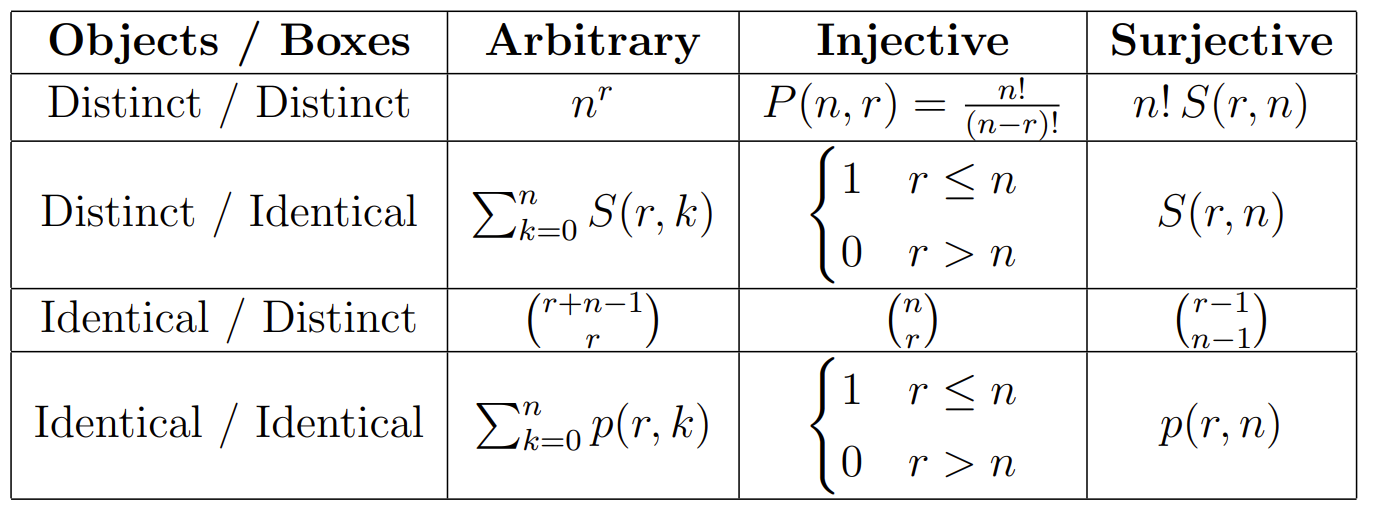
\includegraphics[width=1\linewidth]{twelvefold.png}
\end{center}
\begin{itemize}
    \item Injective / Surjective: Each box has at most / least one object.
    \item $S(r,n)$: Stirling numbers of the second kind.
    \item $p(r, n)$: Number of partitions of $r$ identical objects into exactly $n$ identical boxes.
\end{itemize}

\textbf{Non-Negative Integer Solutions} For the linear equation $x_1+...+x_n=r$ where $x_i\geq 0$, the number of solutions is $H^n_r={n+r-1 \choose r}$ by stars and bars.

\textbf{Multiset} $M=\{r_1\cdot a_1, r_2\cdot a_2,...,r_n\cdot a_n\}$ where $r_i$ is the repetition number of object $a_i$. $\infty \cdot a$ is used to indicate infinite copies of an object.

\textbf{Multiset Permutations} The number of r-permutations of $\{\infty\cdot a_1,...,\infty \cdot a_n\}$ is $n^r$. If $r=\sum_1^n r_i$, the number of permutations of $M$, $P(r;r_1,...,r_n)=\frac{r!}{r_1!...r_n!}$

\textbf{Combinations with Repetition} A $m$ element multi-subset of $M$ is a subset $\{m_1\cdot a_1,...,m_n\cdot a_n\}$ where $\sum_1^nm_i=m$. The number of r-element multi-subsets is given by ${r+n-1 \choose r}$.

\textbf{Stirling Numbers of the Second Kind} $S(r,n)$ or $r \brace n$ counts the number of ways to partition a set of $r$ distinct objects into $n$ \textbf{non-empty}, unlabeled subsets. Base Cases: $S(0,0)=1, S(r,0)=0, r>0, S(0, n)=0, n>0, S(r,n)=0, r <n$. Recursive Definition: $S(r,n)=nS(r-1,n)+S(r-1, n-1)$; either the rth element is in its own subset or it joins an existing subset.

\textbf{Explicit Formula} $S(r,n)=\frac{1}{n!}\sum_{j=0}^n(-1)^{n-j}{n \choose j}j^r$. Derived from $n!\cdot S(r,n)=\sum_{j=0}^n(-1)^j{n \choose j}(n-j)^r$, where LHS is number of surjective functions from $r$ elements to $n$ elements, while RHS is the same by considering PIE on the set of functions avoiding element $i$. $S(n,k)\sim \frac{k^n}{k!}$ as $n \rightarrow \infty$

\textbf{Partitions of an Integer} A partition of $r$ is writing $r$ as a sum of positive integers where \textbf{order does not matter}. The number of partitions of $r$ is $p(r)$, and  $p(r,n)$ if into $n$ sums. $p(n, 2) = \lfloor \frac{n}{2} \rfloor, p(n, 3)=\lfloor \frac{n^2+3}{12}\rfloor$
\begin{itemize}
    \item $p(0,0)=1, p(r,0)=0, r>0, p(0,n)=0,n>0$
    \item $p(r, n)=p(r-1, n-1)+p(r-n, n)$: Either one summand is 1, or all of them are at least 2 so we can subtract 1 from all.
\end{itemize}

% \textbf{Ferrers Diagram} Graphical representation of integer partition as rows of dots or boxes, left-aligned, ordered in non-increasing order.

% \textbf{Conjugate Partition} To get a conjugate partition, we can simply transpose it. The number of partitions of $r$ into $n$ parts is thus the same as the number of partitions of $n$ into $r$ parts.

% \textbf{Polynomials} A polynomial with coefficients in $A$ and variable $x$ is an expression $P(x)=a_nx^n+a_{n-1}x^{n-1}+...+a_1x+a_0$ where $n$ is non-negative, $a_i \in A, a_n \neq 0$.

\textbf{Sequences to Polynomials} $P(x)=a_0+a_1x+...+a_nx^n$ represents the finite sequence $a_n$.

\textbf{Binomial Coefficients} ${n \choose r}=\frac{n!}{r!(n-r)!}$'s are known as the binomial coefficients.

\textbf{Binomial Theorem} $\forall n\geq 0,(x+y)^n=\sum_{r=0}^n{n \choose r}x^{n-r}y^r$. Consider the string of length $n$ with letters $x$ or $y$.

\textbf{Example Identities} $\sum_{r=0}^n {n \choose r}=2^n$ using $(1+1)^n$, $\sum_{r=0}^n(-1)^r{n \choose r}=0$ using $(1+(-1))^n$, ${n \choose 0}+...+{n \choose 2k}={n \choose 1}+...+{n \choose 2k+1}=2^{n-1}$

\textbf{Another Identity} $\sum_{r=1}^n r {n \choose r}=n \cdot 2^{n-1}$ by differentiating $(1+x)^n$ and subbing in $x=1$

\textbf{Multinomial Coefficients} ${n \choose {n_1,n_2,...,n_m}}={n \choose n_1}{n - n_1 \choose n_2}...=\frac{n!}{n_1!n_2!...n_m!}$.

\textbf{Multinomial Theorem} For $n,m \in \mathbb{N}, (x_1+x_2+...+x_m)^n=\sum{n \choose {n_1,n_2,...,n_m}}x_1^{n_1}x_2^{n_2}...x_m^{n_m}$ where we consider all $m$-ary sequences of nonnegative integers summing to $n$.

\section{Ordinary Generating Functions}

% \textbf{Power Series} A power series with coefficients in $A$ and variable $x$ is an expression of the form $\sum_{n=0}^\infty a_nx^n=a_0+a_1x+a_2x^2+...$ where $a_n \in A$. For evaluation it is only valid where $|c|<R$, the radius of convergence.

\textbf{Sequences to Power Series} $F(x)=a_0+a_1x+a_2x^2+...=\sum_{n=0}^\infty a_nx^n$ is the genfunc for the infinite sequence $a_n$.

\textbf{Cauchy Product of Series} The product of two series $F(x)G(x)$ corresponds to the sequence $c=(c_0, c_1, c_2,...), c_r=\sum_{k=0}^ra_kb_{r-k}$. For multiple series, the product corresponds to $c_r=\sum_{k_1+k_2+...+k_m=r}a_{k_1}^{(1)}a_{k_2}^{(2)}...a_{k_m}^{(m)}$.

% \textbf{Encoding Sets} For $A^{(i)}\subseteq \mathbb{Z}_{\geq 0}$, define $F^{(i)}(x)=\sum_{k \in A^{(i)}}x^k$. Let $F(x)=F^{(1)}(x)\cdot...\cdot F^{(m)}(x)$. Then the coefficient $c_r$ of $x^r$ in $F(x)$ counts solutions of $x_1+x_2+...+x_m=r$, $x_i \in A^{(i)}$.

\textbf{Weighted Sums} To count solutions of $x_1+2x_2+...+mx_m=r$, we can use generating functions with weights in exponents. For $x_i$ with coefficient $i$, associate $F^{(i)}(x)=\sum_{k\in A^{(i)}}x^{ik}$. Then $F(x)=F^{(1)}(x)...F^{(m)}(x)$ and the coefficient $c_r$ of $x^r$ counts solutions.

\textbf{Cumulative Sums} Let $F(x)=\sum_{n=0}^\infty a_n x^n$. Then $(1+x+x^2+...)\cdot F(x)=(a_0)+(a_0+a_1)x+...$ encodes $c_r=a_0+...+a_r$.

\textbf{Shifting a Sequence} $x^mF(x)=\sum_{r=0}^\infty c_rx^r$ is the genfunc for the sequence where $c_r=a_{r-m}$. 

\textbf{Constrained Equation} $x_1 \geq 1 \Rightarrow F_1(x)=x+x^2+x^3+..., x_2 \leq 2 \Rightarrow F_2(x)=1+x+x^2$. The genfunc is $F(x)=F_1(x)F_2(x)...$. Then we can use coefficients to find the number of solutions. For $(1+x+...)^2$, the coefficient of $x^k$ is $k+1$.

\textbf{Dividing Genfuncs} Use partial fraction decomposition instead, e.g. $\frac{1}{1-x}=\sum_{n=0}^\infty x^n$, $\frac{1}{1-2x}=\sum_{n=0}^\infty 2^n x^n$.

\textbf{Partition Genfunc} The genfunc for $p(n)$ is $\sum_{n=0}^\infty p(n)x^n=\prod_{k=1}^\infty(1+x^k+x^{2k}+...)=\prod_{k=1}^\infty \frac{1}{1-x^k}$.

\textbf{Euler's Partition Theorem Again} $D(x)=\prod_{k=1}^\infty (1+x^k)$, $O(x)=\prod_{k=1}^\infty \frac{1}{1-x^{2k-1}}$. Using $1+x^k=\frac{1-x^{2k}}{1-x^k}$, we get what we want.

\textbf{Exponential Generating Functions} The EGF for a sequence $(a_r)$ is $a_0+a_1\frac{x}{1!}+...+a_r\frac{x^r}{r!}+...=\sum_{r=0}^\infty a_r\frac{x^r}{r!}$. $a_r=r! c_r$ where $c_r$ is the rth coefficient of the genfunc.

\textbf{OGF v/s EGF} OGF are applicable in distribution or arrangement problems where ordering of objects involved is immaterial. EGF are useful in counting arrangements of objects where ordering is taken into account.

\textbf{General EGF Formula} Let $a_r$ denote the number of r-permutations of the multi-set $\{n_1 \cdot b_1, ... , n_k \cdot b_k\}$. Then the EGF is $(1+\frac{x}{1!}+...+\frac{x^{n_1}_{b_1}}{n_1!})...(1+\frac{x}{1!}+...+\frac{x^{n_k}_{b_k}}{n_k!})$.

\section{Recurrence Relations}

% \textbf{Relating Indexes}
% \begin{itemize}
%     \item ${n+1\choose k}={n \choose k}+{n \choose k-1}$
%     \item $\left[n + 1 \atop k\right]=n \left[n \atop k \right]+\left[n \atop k-1\right]$ (Stirling number of the first type, permutations of $n$ elements with $k$ disjoint cycles)
%     \item $\left \{ n+1 \atop k \right\}=k\left \{ n \atop k \right \}+\left \{n \atop k-1\right\}$ (Stirling number of the second type, partition of $n$ elements into $k$ nonempty subsets)
% \end{itemize}

% \textbf{Recurrence Relation} Relates current term to some previous terms, with base cases known as initial conditions.

% \textbf{Difference Equation} Write in the form $\Delta a_n=a_{n+1}-a_n$.

\textbf{Linear Homogeneous Recurrence Relations} RR with the form $c_0a_n+c_1a_{n-1}+...+c_ra_{n-r}=0$. A function $a_n=f(n)$ solves the RR.

\textbf{Characteristic Equation} For a LHRR, replace $a_i$ by $x^i$, then divide by $x^{n-r}$ to get the characteristic equation. Any root of this equation is a characteristic root.

\textbf{LHRR Theorem} If $\alpha_1,...,\alpha_r$ are the distinct characteristic roots of our RR, then $a_n=A_1(\alpha_1)^n+...+A_r(\alpha_r)^n$ where $A_i$ is constant is the general form of solutions to our RR. Sub in initial conditions to get the solution.

\textbf{Complex Roots} Express using $e^{ix}=cos\ x+isin\ x$.

\textbf{LHRR Theorem Again} If $\alpha_1,...,\alpha_k$ are the distinct characteristic roots such that $\alpha_i$ has multiplicity $m_i$, the general form of the solution of our recurrence relation is $a_n=(A_{11}+A_{12}n+...+A_{1m_1}n^{m_1-1})(\alpha_1)^n+...+(A_{k1}+A_{k2}n+...+A_{km_k}n^{m_k-1})(\alpha_k)^n$.

\textbf{General Linear Recurrence Relation} A recurrence relation of the form $c_0a_n+c_1a_{n-1}+...+c_ra_{n-r}=f(n)$ is an rth order linear recurrence relation. An LHRR is a linear recurrence relation where $f(n)=0$. If $g_1(n), g_2(n)$ are solutions for above, then $h(n)=g_1(n)-g_2(n)$ is a solution of the corresponding LHRR.

\textbf{Solving General Linear Recurrence Relations}
\begin{itemize}
    \item Find the general solution $h(n)$ of the corresponding LHRR.
    \item Find a particular solution $g_0(n)$ of the linear recurrence relation. It can be chosen as a function of a similar type.
    \item The general family of solutions of $g_0(n)$ of the original recurrence relation is given by $g(n)=g_0(n)+h(n)$.
    \item Find the specific solution that fits the given initial conditions.
\end{itemize}

% \textbf{Example Recurrence Relation}
% \begin{itemize}
%     \item Solve $a_n-3a_{n-1}+2a_{n-2}=2^n$ with $a_0=3, a_1=8$
%     \item First solve the LHRR $a_n^{(h)}-3a_{n-1}^{(h)}+2a_{n-2}^{(h)}=0$
%     \item The characteristic equation is $r^2-3r+2=0, r=1,2$
%     \item We get $a_n^{(h)}=A\cdot 1^n + B \cdot 2^n=A+B \cdot 2^n$
%     \item Now find a particular solution by trying $a_n^{(p)}=C \cdot n \cdot 2^n$ since $f(n)=2^n$ and $2$ is a root of the characteristic equation
%     \item Substituting gives us $Cn2^n-3C(n-1)2^{n-1}+2C(n-2)2^{n-2}=2^n$ and solving gives $C=2$
%     \item $a_n^{(p)}=2n \cdot 2^n=n \cdot 2^{n+1}$
%     \item The general solution is $a_n=a_n^{(h)}+a_n^{(p)}=A+B\cdot 2^n+n \cdot 2^{n+1}$
%     \item Applying initial conditions gives $A=2, B=1$
%     \item The final solution is $a_n=2+(2n+1)2^n$
% \end{itemize}

\textbf{$g_0(n)$ Chart}
\begin{itemize}
    \item $Ak^n$, $k$ is not characteristic root: $Bk^n$
    \item $Ak^n$, $k$ is characteristic root with multiplicity $m$: $Bn^mk^n$
    \item $\sum_{i=0}^tp_in^i$, $1$ is not characteristic root: $\sum_{i=0}^tq_in^i$
    \item $\sum_{i=0}^tp_in^i$, $1$ is a characteristic root of multiplicity $m$: $n^m\sum_{i=0}^tq_in^i$
    \item $An^tk^n$, $k$ is not a characteristic root: $(\sum_{i=0}^tq_in^i)k^n$
    \item $An^tk^n$, $k$ is a characteristic root of multiplicity $m$: $n^m(\sum_{i=0}^tq_in^i)k^n$
\end{itemize}

\textbf{Solving Linear Recurrence Relations with GF}
\begin{itemize}
    \item Transform equation into linear equation for generating function
    \item Solve linear equation and simplify the answer, often involving partial fractions
    \item $A(x)-x=\sum a_nx^n=\sum(a_{n-1}+a_{n-2})x^n$, relate the genfunc to the recurrence and express the RHS in terms of $A(x)$, then make it the subject of the formula
    % \item Fibonacci: $a_0=0, a_1=1,a_n=a_{n-1}+a_{n-2}$
    % \item Define $A(x)=\sum_{n=0}^\infty a_nx^n$.
    % \item Then $A(x)-x-0=\sum_{2}^\infty a_nx^n=\sum_{2}^\infty(a_{n-1}+a_{n-2})x^n=x\sum_{1}^\infty a_nx^n+x^2\sum_{0}^\infty a_nx^n=x\cdot A(x) + x^2 \cdot A(x)$.
    % \item We have $A(x)-x=x\cdot A(x)+x^2 \cdot A(x) \Rightarrow A(x)=\frac{x}{1-x-x^2}$.
    % \item We have $1-x-x^2=(1-r_1x)(1-r_2x)$, and $A(x)=\frac{1}{\sqrt{5}}(\frac{1}{1-r_1x}-\frac{1}{1-r_2x})$. Then we get $a_n=\frac{1}{\sqrt{5}}(r_1^n-r_2^n)$ by comparing coefficients.
\end{itemize}

\textbf{Partial Fractions}
\begin{itemize}
    \item Distinct Linear Factors: $\frac{P(x)}{(1-r_1x)(1-r_2x)...(1-r_kx)}=\sum_{i=1}^k\frac{A_i}{1-r_ix}$
    \item Each term expands as $\frac{1}{1-rx}=\sum_{n=0}^\infty r^n x^n$
    \item Repeated Roots: Multiplicity $m$: $\frac{P(x)}{(1-rx)^m}=\frac{B_1}{1-rx}+...+\frac{B_m}{(1-rx)^m}$
    \item Expansion gives terms of the form $\frac{1}{(1-rx)^j}=\sum_{n=0}^\infty{n+j-1 \choose j-1} r^nx^n$
    \item Use $x=\frac{1}{r_i}$ to eliminate and solve for other coefficients
\end{itemize}

\textbf{System of Linear Recurrence Relations}
\begin{itemize}
    \item Domino Tiling: Tile $2 \times n$ board using $1 \times 2$ and $1 \times 1$ tiles
    \item Let $a_n$ be complete tilings, and $b_n$ be tilings with a missing square
    \item $a_n=b_n+a_{n-1}+b_{n-1}+a_{n-2}$
    \item $b_n=a_{n-1}+b_{n-1}$
    \item Use substitution to eliminate one sequence, then spam genfunc
\end{itemize}

\section{Tutorial Stuff}
\textbf{More Identities}
\begin{itemize}
    \item $P_r^n=nP_{r-1}^{n-1}$, $P_r^n=(n-r+1)P_{r-1}^n$
    \item $P_r^n=\frac{n}{n-r}P_r^{n-1}$, $P_r^{n+1}=P_r^n+rP_{r-1}^n$
    \item $P_r^{n+1}=r!+r(P_{r-1}^n+P_{r-1}^{n-1}+...+P_{r-1}^r)$: Either take the last $r$ elements, or place $n+1$, don't take $n+1,n,n-1,...,i+1$, then take $i$
\end{itemize}

\textbf{Divisibility Argument}
\begin{itemize}
    \item Prove $(n+1)(n+2)...(2n)$ is divisible by $2^n$
    \item Pairing $2n$ people tells us $\frac{(2n)!}{n!\cdot2^n}$ is an integer. So $\frac{(2n)!}{n!\cdot2^n} \cdot 2^n$ which is what we want is also an integer.
\end{itemize}

\textbf{Even Function} For any function $f(k)$, $\sum_{\text{even } k} f(k)=\sum_{k=0}^n\frac{1^k+(-1)^k}{2}f(k)$

\textbf{Power Series} $\frac{1}{(1-x)^r}=\sum_{n=0}^\infty {n+r-1 \choose r-1}x^n=\sum_{n=0}^\infty H^r_nx^n$, $1+x+x^2+...+x^n=\frac{1-x^{n+1}}{1-x}$, $1+x^n=\frac{1-x^{2n}}{1-x^n}$

\textbf{Generalised Binomial Theorem} ${n \choose r} = \frac{n(n-1)...(n-r+1)}{r!}$.

% \subsection{Some Combinatorial Identities}
% \textbf{ID1} $\sum_{r=0}^n{n \choose r}=2^n$ using $(1+1)^n$.

% \textbf{ID2} $\sum_{r=0}^n(-1)^r{n \choose r}={n \choose 0}-{n\choose 1}+...+(-1)^n{n \choose n}=0$ using $(1-1)^n$.

% \textbf{ID3} ${n\choose 0}+{n \choose 2}+...+{n \choose 2k}+...={n \choose 1}+{n \choose 3}+...+{n \choose 2k+1}+...=2^{n-1}$ by differentiating binomial theorem.

% \textbf{ID4} $\sum_{r=1}^nr{n \choose r}=n\cdot 2^{n-1}$.

% \textbf{ID5} $\sum_{r=1}^n r^2{n \choose r}=n(n+1)2^{n-2}$ by double differentiating binomial theorem.

% \textbf{Example 5.8} $\sum_{r=1}^n r^3{n \choose r}=n^2(n+3)2^{n-3}$.

% \textbf{Example 5.9} $\sum_{r=0}^n(-1)^rr{n \choose r}=0$.

% \textbf{Example 5.10} $\sum_{r=0}^{n-1}{2n-1\choose r}=2^{2n-2}$.

% \textbf{Example 5.11} $\sum_{r=0}^n{2n \choose r}=2^{2n-1}+\frac{1}{2}{2n \choose n}$.

\textbf{Vandermonde's Identity} $\sum_{i=0}^r{m \choose i}{n \choose r-i}={m\choose 0}{n \choose r}+{m \choose 1}{n \choose r-1}+...+{m \choose r}{n \choose 0}={m+n \choose r}$ using $(1+x)^{m+n}=(1+x)^m(1+x)^n$.

\textbf{Derangments} $!n=n!-{n \choose 1}(n-1)!+{n \choose 2}(n-2)!...$

\section{Graph Theory}
\textbf{Graph} Collection of vertices and edges; Finite, undirected, simple, with no loops. Denoted by $G=(V, E)$ where $V(G)$ is the vertex set and $E(G)$ is the edge set. $uv \in E(G), u \sim v$ is an edge. $v(G)=|V(G)|, e(G)=|E(G)|$.

\textbf{Identical and Isomorphic Graphs} $G, H$ are identical if $V(G)=V(H), E(G)=E(H)$. $G \cong H$ if there is a bijection $f:V(G)\rightarrow V(H), u \sim v \in G \Leftrightarrow f(u) \sim f(v) \in H$. This is an equivalence relation.

\textbf{Complement} $\overline{G}$ is the complement of $G$ with the same vertex set $V(G)$ and edge set ${V(G) \choose 2} \backslash E(G)$.

\textbf{Complete Graph} $K_n$ is the complete graph with $n$ vertices and $n \choose 2$ edges.

\textbf{Petersen Graph} Star connected to pentagon. 10 vertices, 15 edges, $deg(i)=3$.

\textbf{Hypercube Graph} $Q^d$, vertices are $\{0,1\}^d$, and edges are a bit flip, has $2^d$ vertices, $d \cdot 2^{d-1}$ edges.

\textbf{Subgraph} $H$ is a subgraph of $G$ if $V(H) \subset V(G), E(H) \subset E(G)$, $E(H) \subset {V(H) \choose 2}$. A spanning subgraph has $V(H)=V(G)$ ($2^{n \choose 2}$ of them). An induced subgraph $G[S]$ on $S \subset V(G)$ has vertex set $S$ and all edges from $G$ with both endpoints in $S$ ($2^n$ of them). There are $\sum_{k=0}^n {n \choose k}2^{k \choose 2}$ subgraphs.

\textbf{Adjacency Matrix} $n\times n$ symmetric matrix where $A_{i,j}=1$ if $v_iv_j \in E(G)$, $0$ otherwise. Diagonal entries are zero.

\textbf{Incidence Matrix} $v$ is incident to $e$ if $v \in e$. $n \times m$ matrix where $M_{i,j}=1$ if $v_i$ is incident to $e_j$, $0$ otherwise. Columns represent edges.

\textbf{Relation between Representations} $M_GM_G^T=diag(d(v_1),...,d(v_n))+A_G$.

\textbf{Number of Graphs} ${{n \choose 2} \choose m}$ labeled graphs. Asymptotically $/n!$ for unlabeled.

\textbf{Neighbourhood} $N(v)$ is the set of all $u$ adjacent to $v$.

\textbf{Degree} $d(v)=|N(v)|$. Degree sequence: List of all vertex degrees, often sorted in non-increasing order. $\delta(G)$: smallest degree, $\Delta(G)$: largest degree, k-regular: all vertices have degree $k$. $\overline{d}(G)=\frac{1}{|V(G)|}\sum_{v \in V(G)}d(v)$: average degree.

\textbf{Handshake Lemma} $\sum_{v \in V(G)}d(v)=2e(G)$. $\overline{d}(G)=\frac{2e(G)}{v(G)}$. The number of odd degree vertices is even.

\textbf{Bipartite Graph} A graph is bipartite if $V=A \cup B, A \cap B = \emptyset$, there are no edges within $A$ or $B$. A k-regular bipartite graph has $|A|=|B|$.

\textbf{Graphic Sequences} Degree sequence of some graph.

\textbf{Havel-Hakimi Theorem} The non-increasing sequence $(d_1,...,d_n)$ is graphic iff $(d_2-1, d_3-1,...,d_{d_1+1}-1,d_{d_1+2},...,d_n)$ is graphic. Repeatedly remove largest degree $d_1$ and subtract $1$ from the next $d_1$ degrees, until obvious.

\textbf{Erdős-Gallai Theorem} A non-increasing sequence is graphic iff it has an even sum and for all $k \in \{1,...,n\}, \sum_{i=1}^k d_i \leq k(k-1)+\sum_{i=k+1}^n min\{d_i,k\}$.

\textbf{Cliques} $\omega(G)$ is the number of vertices in the largest clique of $G$. $\alpha(G)$ is the size of the largest independent set in $G$. $\alpha(G)=\omega(\overline{G}), \omega(G)=\alpha(\overline{G})$.

\textbf{Graph Families} $C_n$: cycle, $P_n$: path, $K_{m,n}$: complete bipartite.

\textbf{Kneser Graph} $KG(n,k)$ is the graph where vertices are all k-element subsets of $n$ and edges are between disjoint k-subsets. 

\textbf{Erdős-Ko-Rado Theorem} For $n \geq 2k$, $\alpha(KG(n,k))={n-1 \choose k-1}$.

\textbf{Graph Colourings} A proper $k$-Colouring is $c:V(G)\rightarrow\{1,...,k\}$ such that $uv \in E(G) \Rightarrow c(u) \neq c(v)$. The chromatic number $\chi(G)$ is the smallest $k$ such that $G$ has a proper $k$-colouring.

\textbf{Lovász's Theorem} $\chi(KG(n,k))=n-2k+2$.

\textbf{Bounding Chromatic Number} For every $G$, $\chi(G) \geq \omega(G), \chi(G) \geq \frac{|V(G)|}{\alpha(G)}$. For $m$ edges, $\chi(G) \leq \frac{1}{2}+\sqrt{2m+\frac{1}{4}}$. $\chi(G) \leq \Delta(G)+1$.

\textbf{Walks} For length $k$, non-empty alternating sequence $v_0,e_0,...,e_{k-1}, v_k$ with $e_i=\{v_i,v_{i+1}\}\in E(G)$. If $v_0=v_k$, the walk is closed.

\textbf{Connectedness} All pairs have a walk between them, equivalence relation.

\textbf{Connected Component} Partition of $V(G)$ based on connectedness.

\textbf{Counting Walks} $(A^k)_{ij}$ gives the number of walks of length $k$ from $i$ to $j$.

% \textbf{Spectral Analysis} Let the adjacency matrix have eigenvalues $\lambda_1,...,\lambda_n$. The number of closed walks of length $k$ is $tr(A^k)=\sum_{i=1}^n \lambda_i^k$. It grows roughly with $\rho(A)^k$ where $\rho(A)=max_i|\lambda_i|$ is the spectral radius. For a graph with $|x| < 1/\rho(A)$, $(I-xA)^{-1}=\sum_{k=0}^\infty x^kA^k$ gives a genfunc for walk counts between $i$ and $j$. The diagonal entries give the same for closed walks.

\textbf{Connected Components} Let $D$ be the diagonal matrix of degrees. The Laplacian matrix of $G$ is $L=D-A$. Then the number of connected components of $G$ is $nullity(L)$ (number of free variables in RREF).

\textbf{Paths and Trails} A trail is a walk with no repeated edges. If a walk or trail has no repeated vertices, it is a path. Every $u-v$ walk contains a $u-v$ path.

\textbf{Distance} $d_G(x, y)$ is the length of a shortest path connecting $x$ and $y$, $\infty$ if it does not exist.

% This defines a metric on $V(G)$ which satisfies the following:
% \begin{enumerate}
%     \item $d(x,y) \geq 0, d(x, y) = 0 \Leftrightarrow x = y$
%     \item $d(x, y)=d(y,x)$
%     \item $d(x,z) \leq d(x, y) + d(y,z)$
% \end{enumerate}

\textbf{Diameter} $diam(G)=max_{x,y \in V(G)}d(x,y)$.

\textbf{Breadth First Search} Expand layer by layer by adding each set of undiscovered neighbours to the search frontier.

\textbf{Vertex Cut} $S \subset V(G)$, $G-S$ is disconnected. If $|S|=1$, it is a cut vertex.

\textbf{Vertex Connectivity} $\kappa(G)=\min\{|S|:S \subseteq V(G), G-S\text{ is disconnected }\}$. $k$-connected: $\kappa(G) \geq k$ or deleting $k-1$ vertices leaves it connected.

\textbf{Girth / Circumference} Minimum / Maximum length of cycle contained in $G$.

\textbf{Acyclic Graph} Graph with no cycle as a subgraph.

\textbf{Cycle Proposition} Every 2-connected graph contains a cycle.

\textbf{r-Partite} $G$ is r-partite if it can be partitioned into $V(G)=V_1\cup...\cup V_r$.

\textbf{Bipartite Proposition} A graph is bipartite iff it contains no odd cycles.

\textbf{Eulerian Circuit} Closed trail using every edge exactly once.

\textbf{Euler's Theorem} A graph is Eulerian iff all vertices have even degrees.

\textbf{Depth First Search} Recursively visit every unvisited neighbour before backtracking. Find cycles by checking for back edges to already visited nodes.

\textbf{Hamiltonian} A Hamiltonian cycle is a closed walk that visits every vertex exactly once. Path is similar. $Q^n$ is Hamiltonian, while the Petersen graph is not.

\textbf{Dirac's Theorem} If $G$ has $n \geq 3$ and $\delta(G) \geq n/2$, then $G$ is Hamiltonian. For even $n$, if $\delta(G) \geq n/2$, then $G$ has a perfect matching.

\textbf{Ore's Theorem} If $G$ has $n \geq 3$ and every non-adjacent pair $u,v$ satisfies $deg(u)+deg(v) \geq n$, then $G$ is Hamiltonian.

\textbf{Closure} Add edges where non-adjacent $u,v$ have $deg(u)+deg(v) \geq n$.

\textbf{Bondy-Chvátal Theorem} $G$ is Hamiltonian iff its closure $Cl(G)$ is Hamiltonian.

\textbf{Forest / Tree} Acyclic Graph. A tree is a connected forest.

\textbf{Leaf} Vertex with degree $1$. Removal does not disconnect the graph.

\textbf{Characterisations of Trees} TFAE
\begin{enumerate}
    \item $T$ is a tree.
    \item Any two vertices of $T$ are connected by a unique path in $T$.
    \item $T$ is minimally edge connected (removal of any edge disconnects the tree).
    \item $T$ is maximally acyclic (acyclic but any new edge creates a cycle).
    \item $T$ is a connected graph on $n$ with $n-1$ edges.
\end{enumerate}

\textbf{Vertex Ordering} The vertices of a tree $T$ can be ordered such that the ith vertex $v_i$ has a unique neighbour in $\{v_1,...,v_{i-1}\}$. Every tree has at least one leaf. A connected graph on $n$ vertices is a tree iff it has $n-1$ edges.

\textbf{Embedding Trees} If $T$ is a tree on $k$ vertices, and $G$ is a graph with $\delta(G) \geq k-1$, then $G$ contains a subgraph isomorphic to $T$.

\textbf{Erdős-Sós Conjecture} Every graph $G$ on $n \geq k$ vertices having average degree $d(G) > k-2$ must contain every tree of $k$ vertices.

\textbf{Rooted Tree} Tree with a fixed vertex called the root.

\textbf{Spanning Tree} Subgraph that is a tree and includes all vertices of $G$. Every connected graph $G$ has a spanning tree.

\textbf{BFS/DFS Tree} Spanning tree obtained by exploring a graph level by level from a root vertex / exploring as far as possible along each branch before backtracking.

% \textbf{Weighted Graph} A graph with a weight function $w: E \rightarrow \mathbb{R}$.

\textbf{Minimum Spanning Tree} Spanning tree $T$ minimising $w(T)=\sum_{e \in E(T)} w(e)$.

\textbf{Safe Edge} Let $A$ be a set of edges included in a MST that is being built. An edge is safe if $A \cup \{(u,v)\}$ is a subset of some final MST.

\textbf{Cut Property} Let $A$ be a subset of some MST. For any cut $(S, V-S)$ that respects $A$, if $e$ is a minimum weight edge crossing the cut, then $e$ is safe for $A$.

\textbf{Kruskal's Algorithm} Sort edges by non-decreasing weight. Then for each edge, if adding it does not create a cycle, add it to the MST.

\textbf{Prim's Algorithm} Start from an arbitrary vertex. Then repeatedly add the minimum weight edge that connects to new vertices.

\textbf{Cycle Property} For any cycle $C$ the maximum weight edge $e$ is not in any MST.

\textbf{Reverse-Delete Algorithm} Start with all edges, sorted in non-increasing order. Then for each edge, if the graph without the edge is still connected, remove it.

\textbf{Cayley's Theorem} The number of distinct labeled trees on $n$ vertices is $n^{n-2}$.

\textbf{Prüfer Code}
\begin{itemize}
    \item Bijection between labeled trees on $n$ vertices and sequences of length $n-2$ with entries from $\{1,...,n\}$.
    \item Encoding: Repeatedly find the leaf with the smallest label, add its neighbour to the set, then remove the leaf.
    \item Decoding: Repeatedly find smallest element not in the sequence $P$, then add edge between it and the first element of $P$, then remove both.
\end{itemize}

\textbf{Degree Sequence Formula} The the number of labeled trees on $n$ vertices is $\frac{(n-2)!}{(d_1-1)!...(d_n-1)!}$ by multinomial coefficients.

% \textbf{Laplacian Matrix Properties}
% \begin{enumerate}
%     \item All rows sum to 0.
%     \item Symmetric.
%     \item Positive semidefinite.
%     \item Multiplicity of eigenvalue 0 is equal to the number of connected components.
% \end{enumerate}

\textbf{Cofactor} The $(i,j)$-cofactor of a matrix is $(-1)^{i+j}$ times the determinant of the submatrix obtained by deleting row $i$ and column $j$.

\textbf{Kirchhoff's Matrix Tree Theorem} The number of spanning trees equals any cofactor of the Laplacian matrix $L(G)$. $\tau(G)=(-1)^{i+j}det(L_{ij})$ where $L_{ij}$ is $L$ with row $i$ and column $j$ deleted.

\textbf{Oriented Incidence Matrix} $n\times m$ matrix where each column corresponds to an edge and for edge $(i,j)$, put $+1$ in row $i$, $-1$ in row $j$, and 0 elsewhere.

\textbf{Incidence Matrix and Laplacian} $L=DD^T$

\textbf{Binet-Cauchy Theorem} If $A, B$, are $n \times m$ with $m \leq n$, then $det(AB)=\sum_{S\subseteq [n], |S|=m} det(A_{[m]},S)det(B_S,[m])$ where the sum is over all $m$-element subsets of columns.

\textbf{Kirchhoff Lemma} For the incidence matrix with one row deleted; for any subset $S$ of $n-1$ edges, $det(D_S)=\pm 1$ if $S$ forms a spanning tree or 0 otherwise.

\textbf{Weighted Matrix Tree Theorem} For a weighted graph, the sum of weights of all spanning trees where tree weight = product of edge weights equals any cofactor of the weighted Laplacian $L_{ij}= \sum_{k \neq i} w_{ik}$ if $i=j$, $-w_{ij}$ otherwise.

% \textbf{Reliability Polynomial} The probability that a network remains connected when edges fail independently with probability $p$ is given by $R(G,p)=\sum_{T \text{ is a spanning tree}}p^{n-1}(1-p)^{m-n+1}+\text{higher terms}$.

\epigraphwidth=0.9\columnwidth
\epigraph{This question is evil, but it's okay because I am evil.}{\textit{Tran Chieu Minh, 2025}}

\end{multicols*}

\end{document}